% Chapter Template

\definecolor{mybluei}{RGB}{124,156,205}
\definecolor{myblueii}{RGB}{73,121,193}
\definecolor{mygreen}{RGB}{202,217,126}
\definecolor{mypink}{RGB}{233,198,235}

% this length is used to control the width of the light blue frame
% for the upper part of the diagram
\newlength\myframesep
\setlength\myframesep{8pt}

\pgfdeclarelayer{background}
\pgfsetlayers{background,main}

\pgfkeys{
    /tikz/node distance/.append code={
        \pgfkeyssetvalue{/tikz/node distance value}{#1}
    }
}

\newcommand\widernode[5][blueb]{
\node[
        #1,
        inner sep=0pt,
        shift=($(#2.south)-(#2.north)$),
        yshift=-\pgfkeysvalueof{/tikz/node distance value},
        fit={(#2) (#3)},
        label=center:{\sffamily\bfseries\color{white}#4}] (#5) {};
}

\chapter{\robotto} % Main chapter title

\label{Chapter2} % Change X to a consecutive number; for referencing this chapter elsewhere, use \ref{ChapterX}

\lhead{Cap\'itulo 2. \emph{\robotto}} % Change X to a consecutive number; this is for the header on each page - perhaps a shortened title

%----------------------------------------------------------------------------------------
%	SECTION 1
%----------------------------------------------------------------------------------------

Ahora que se conoce la finalidad de \robotto se procederá a explicar su funcionamiento, sus partes, y como estas se relacionan entre sí

\section{Diseño de \robotto}

A lo largo de esta sección se explicarán las distintas decisiones en el diseño de \robotto. Tal y como se aprecia en el esquema principal, ver \ref{fig:Esquema}, se buscan varios objetivos.\\
Por una parte se quiere poder portar desde un software de edición 3D como blender a un formato propio y este a su vez que sea fácil de editar proporcionando un editor capaz de ello. \\
Por otra parte se busca desacoplar la interfaz que usará el usuario del núcleo del motor proporcionando así seguridad de uso y una interfaz estable abierta a la extensión pero cerrada a la modificación.\\
Además, y tal y como se espera de un motor de gráficos 3D, está la gestión de la escena y de los recursos para una correcta visualización.\\
Y por último, pero no menos importante, la capacidad de interactuar con eventos procedentes del dispositivo.\\

\begin{figure}[h!]
\begin{center}
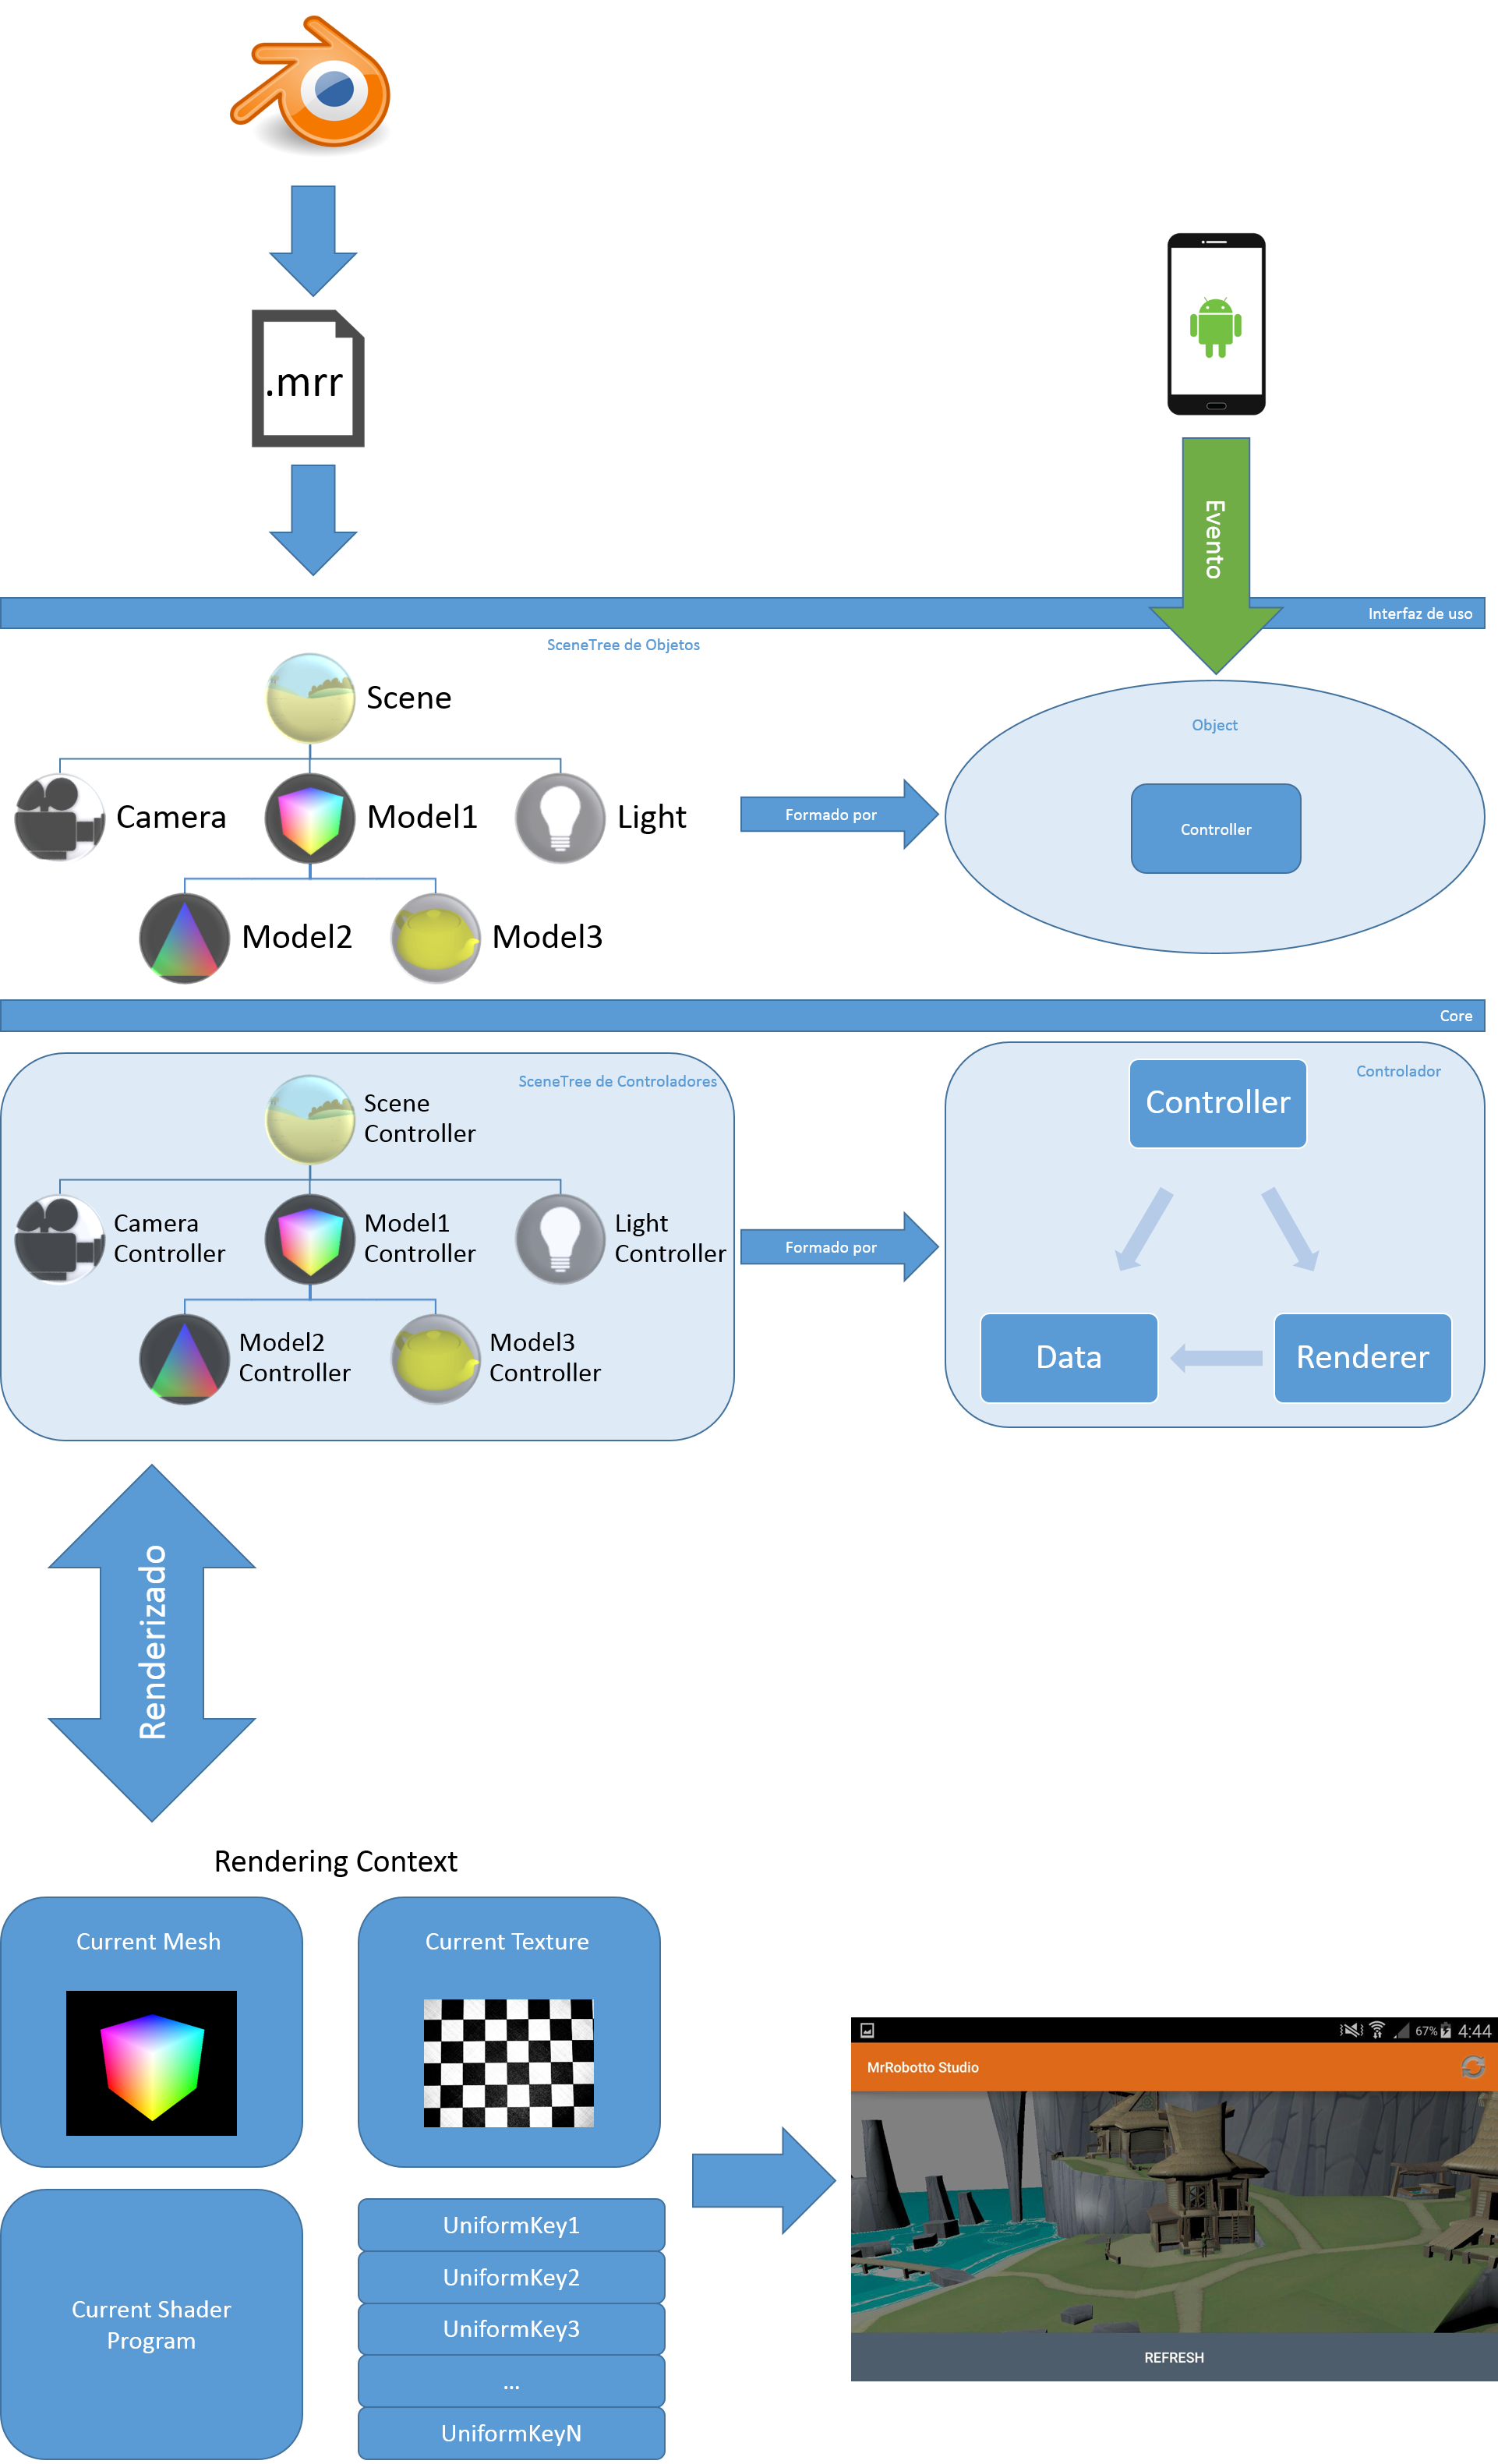
\includegraphics[scale=0.4]{esquema.png}
\end{center}
\caption[Esquema principal de \robotto]{Esquema principal de \robotto}
\label{fig:Esquema}
\end{figure}

\subsection{Formato .MRR}
La decisión de usar un formato propio frente a usar alguno ya ampliamente aceptado como podría ser \textit{.fbx} o \textit{.dae} viene fomentado por la necesidad de controlar en su totalidad los distintos datos y sobretodo, la forma en la que estos se almacenarán dentro de una aplicación.\\

Por ejemplo de cara al rendimiento se decidió almacenar los vértices de forma intercalada tal y como se recomienda en \cite{1misc} a la vez que usar en todo momento \textit{Index Buffer Objects} como se recomienda en \cite{2misc}.\\
También se tomó en cuenta la necesidad de modificar la configuración de cómo se mostrará la escena sin necesidad de código, si no la realización de esta mediante un fichero. Por ejemplo, gracias al formato MRR se puede decidir si una malla va a ser dibujada usando triángulos o bien líneas únicamente.\\

Aún así estas no son las únicas razones para proporcionar un formato propio, algunas de las citadas configuraciones podrían llevarse a cabo fácilmente haciendo uso de otros tipos de formatos más comunes. El mayor motivo detrás de la creación del formato MRR es la creación de un formato que fuera \textit{Scene Object Centric}.\\
Con este término, \textit{Scene Object Centric}, se hace alusión a un diseño centrado en los objetos de la escena, donde cada elemento es independiente del resto de elementos que pudiesen estar definidos en ella. De esta forma la tarea de comunicar un objeto con otro recae sobre el motor y no es arrastrada desde el formato.
Únicamente hay un único punto de conexión entre los objetos y este se realiza mediante los denominados \hyperref[susec:UnifKeyUnifGen]{UniformKeys y UniformsGenerators}

Toda la información acerca del formato y cómo está organizada la información almacenada en él puede verse en \ref{AppendixA}

\subsection{El SceneTree}
El SceneTree es la estructura fundamental de almacenamiento de los objetos de la escena.\\
Posee una estructura de árbol donde cada nodo puede tener un número variable de hijos, pero lo que lo diferencia de una estructura de árbol normal es que sus nodos se encuentran indexados tanto por el nombre del dato almacenado en el nodo como por su tipo, permitiendo así realizar búsquedas dentro de la estructura en $O(1)$\\
Su funcionamiento se explicará de forma detallada en \ref{susec:MrSceneTree}

\subsection{Elementos de una Escena}
Para los elementos constituyentes de una escena 3D se decidió emular el diseño de componentes de otros motores 3D a la vez que la necesidad de que la API fuese lo más sencilla y funcional que se pudiera.\\

\subsubsection{Object}
Los objetos genéricos tienen la función de ser la base de la jerarquía del resto de objetos de la escena, y en él ser verán reflejados todas las acciones compartidas. A saber:

\begin{itemize}
\item Gestión de las transformaciones geométricas:\newline
Se espera que un objeto de una escena pueda ser transformado por traslaciones, rotaciones y escalados dentro de la escena que los contiene.
\item Inicialización:\newline
La inicialización de los objetos de la escena hace referencia a varias acciones que deben ser llevadas a cabo antes del uso del objeto, a saber estas pueden ser:
\begin{itemize}
\item Establecimiento del comportamiento de los objetos frente a los eventos
\item Configuración de ciertos elementos en la GPU, como podría ser iniciar un Vertex Buffer Object.
\item Configuración previa dependiente del tamaño de la ventana donde va a realizarse el dibujado de la escena, como por ejemplo, la creación de la matriz de proyección.
\end{itemize}
\item Actualización de los diferentes elementos que dependen de él en cada ciclo de renderizado, como podría ser la gestión de eventos o envío de datos a la GPU
\item Métodos de comunicación con la escena y otros objetos
\end{itemize}

\subsubsection{Model}
Los modelos 3D son seguramente los elementos más representativos dentro del motor puesto que son los únicos elementos realmente visibles de la escena.\\
Los modelos no representan únicamente las mallas tridimensionales visibles en el mundo, si no que además engloba otras funcionalidades tales como

\begin{itemize}
\item Gestión de la visualización final:\\
Un modelo será capaz de gestionar como será su aspecto final en la escena, es decir, un modelo será capaz de hacer uso de un sombreador (\textit{Shader}) independiente al resto.
\item Gestión de las animaciones:\\
En el caso de que el modelo tuviera animaciones basadas en esqueleto, es el modelo quien tiene el control sobre este.\\
En otros motores los esqueletos suelen manejarse de forma independiente al resto de elementos y como un objeto de la escena más, pero en el caso de \robotto se decidió que un esqueleto carece de sentido si no existe un modelo sobre el cuál se aplique.
\item Gestión de materiales y texturas:\\
Las texturas y materiales utilizados en cada modelo, aunque puedan ser compartidos entre multipes modelos, es tarea de cada uno el controlar la textura o material usado en cada momento.
\end{itemize}

\subsubsection{Cámaras y Luces}
La cámara es el objeto de escena encargado de proporcionar el punto de vista a través del cual será visualizado el mundo.\\
Además de ello también ofrece el tipo de proyección a utilizar, a escoger entre ortogonal y perspectiva.\\

Por otra parte las luces son los objetos de la escena encargados de proporcionar la iluminación. Las luces soportadas actualmente por \robotto se reducen a luces puntuales aunque resulta fácilmente ampliable a otro tipo de luces.\\

\subsubsection{Scene}
Posiblemente este es el objeto más conflictivo conceptualmente ya que no parece posible que la escena sea considerada como un objeto de la escena, sin embargo hay una justificación para esta decisión.\\
Aunque la escena no genere estrictamente hablando un cambio visible si se decide hacer una transformación geométrica sobre ella, o al reaccionar frente a un evento, la finalidad de que sea considerada como objeto de la escena es que de esa manera es posible configurar algunos aspectos visibles con datos procedentes desde el fichero MRR. Es decir, de esta forma algunos atributos como por ejemplo el color plano con el que se limpia la escena puede cambiarse en la configuración y no desde código.\\
Aún así existen más motivos que justifican esta decisión, y es que la escena, conceptualmente, es un buen lugar donde albergar la responsabilidad de la generación de uniforms que sean dependientes de varios objetos. Este concepto se explica en la siguiente apartado.

\subsection{Los Conceptos de UniformKey y UniformGenerator}\label{susec:UnifKeyUnifGen}
En este apartado se tratará cómo se realiza el envío de datos desde CPU a la GPU.\\
Antes de comenzar se introducirán algunos términos referidos a la programación gráfica, por una parte se ha de conocer que es un Shader Program. Un Shader Program es un programa orientado a ser ejecutado sobre la GPU y que se encarga de realizar el sombreado sobre los distintos vértices de los objetos renderizados.\\
Dichos Shader Programs pueden recibir entradas de datos, estos se dividen en Attributes, que son datos dependientes de cada vértice y Uniforms, que son datos constantes dentro de cada ejecución del Shader Program, siendo así independientes de los vértices.

Ahora bien, una vez introducidos los conceptos, con el fin de enviar los Uniforms desde CPU a GPU de forma sencilla se han implementado en \robotto tres elementos muy relacionados entre sí.\\
\begin{itemize}
\item En primer lugar se tienen los \textbf{Uniforms}, que no son si no una representación de los \textit{uniforms} usados en los \textit{Shader Programs}.\\
Dichos Uniforms poseen, entre otras cosas, dos campos fundamentales que hacen posible la comunicación
\begin{itemize}
\item El \texttt{UniformType}, que determina el tipo uniform al que se hace referencia, como podría ser la matriz de proyección o la \textit{ModelView Matrix}.\\
Podría pensarse que este papel ya es desempeñado por el nombre del uniform dentro del \textit{Shader Program}, sin embargo, definiendo el tipo del Uniform de esta forma permite que distintos \textit{Shader Programs} puedan requerir un mismo Uniform sin necesidad de que su código presente las mismas variables obligatoriamente.
\item El \texttt{UniformId} representa el identificador dado por la GPU a la variable \textit{uniform} en cuestión.
\end{itemize}
\item Por otra parte se tienen los \textbf{UniformGenerators}, estos elementos tienen como función principal asignarle a cada objeto la funcionalidad necesaria para generar los valores de los Uniforms que este objeto sea el encargado de producir. Por ejemplo, la cámara será la encargada de producir la \textit{View Matrix} pero no la \textit{Model View Matrix} ya que esta depende de la cámara y también de la \textit{Model Matrix}, la cuál es generada por un modelo.\\
Todo UniformGenerator poseerá un identificador único dentro del conjunto de generadores de un objeto individual.
\item Por último está el elemento que actúa como puente entre los dos anteriormente detallados, los \textbf{UniformKeys}.\\
Entre las funciones de los UniformKeys las más destacables son:
\begin{itemize}
\item Almacenar el valor de los uniforms generados en los UniformGenerators.
\item Proporcionar información acerca de los uniforms que un objeto es capaz de generar.\\
De esta última afirmación se deduce que todo UniformKey ha de tener asociado obligatoriamente un UniformGenerator
\end{itemize}
Para conseguirlo el UniformKey cuenta con un campo que le permite enlazarse con el objeto Uniform, el ya comentado \texttt{UniformType} y por otra parte, otro campo que le permita comunicarse con su UniformGenerator asociado.
\end{itemize}

\begin{figure}[h!]
\begin{center}
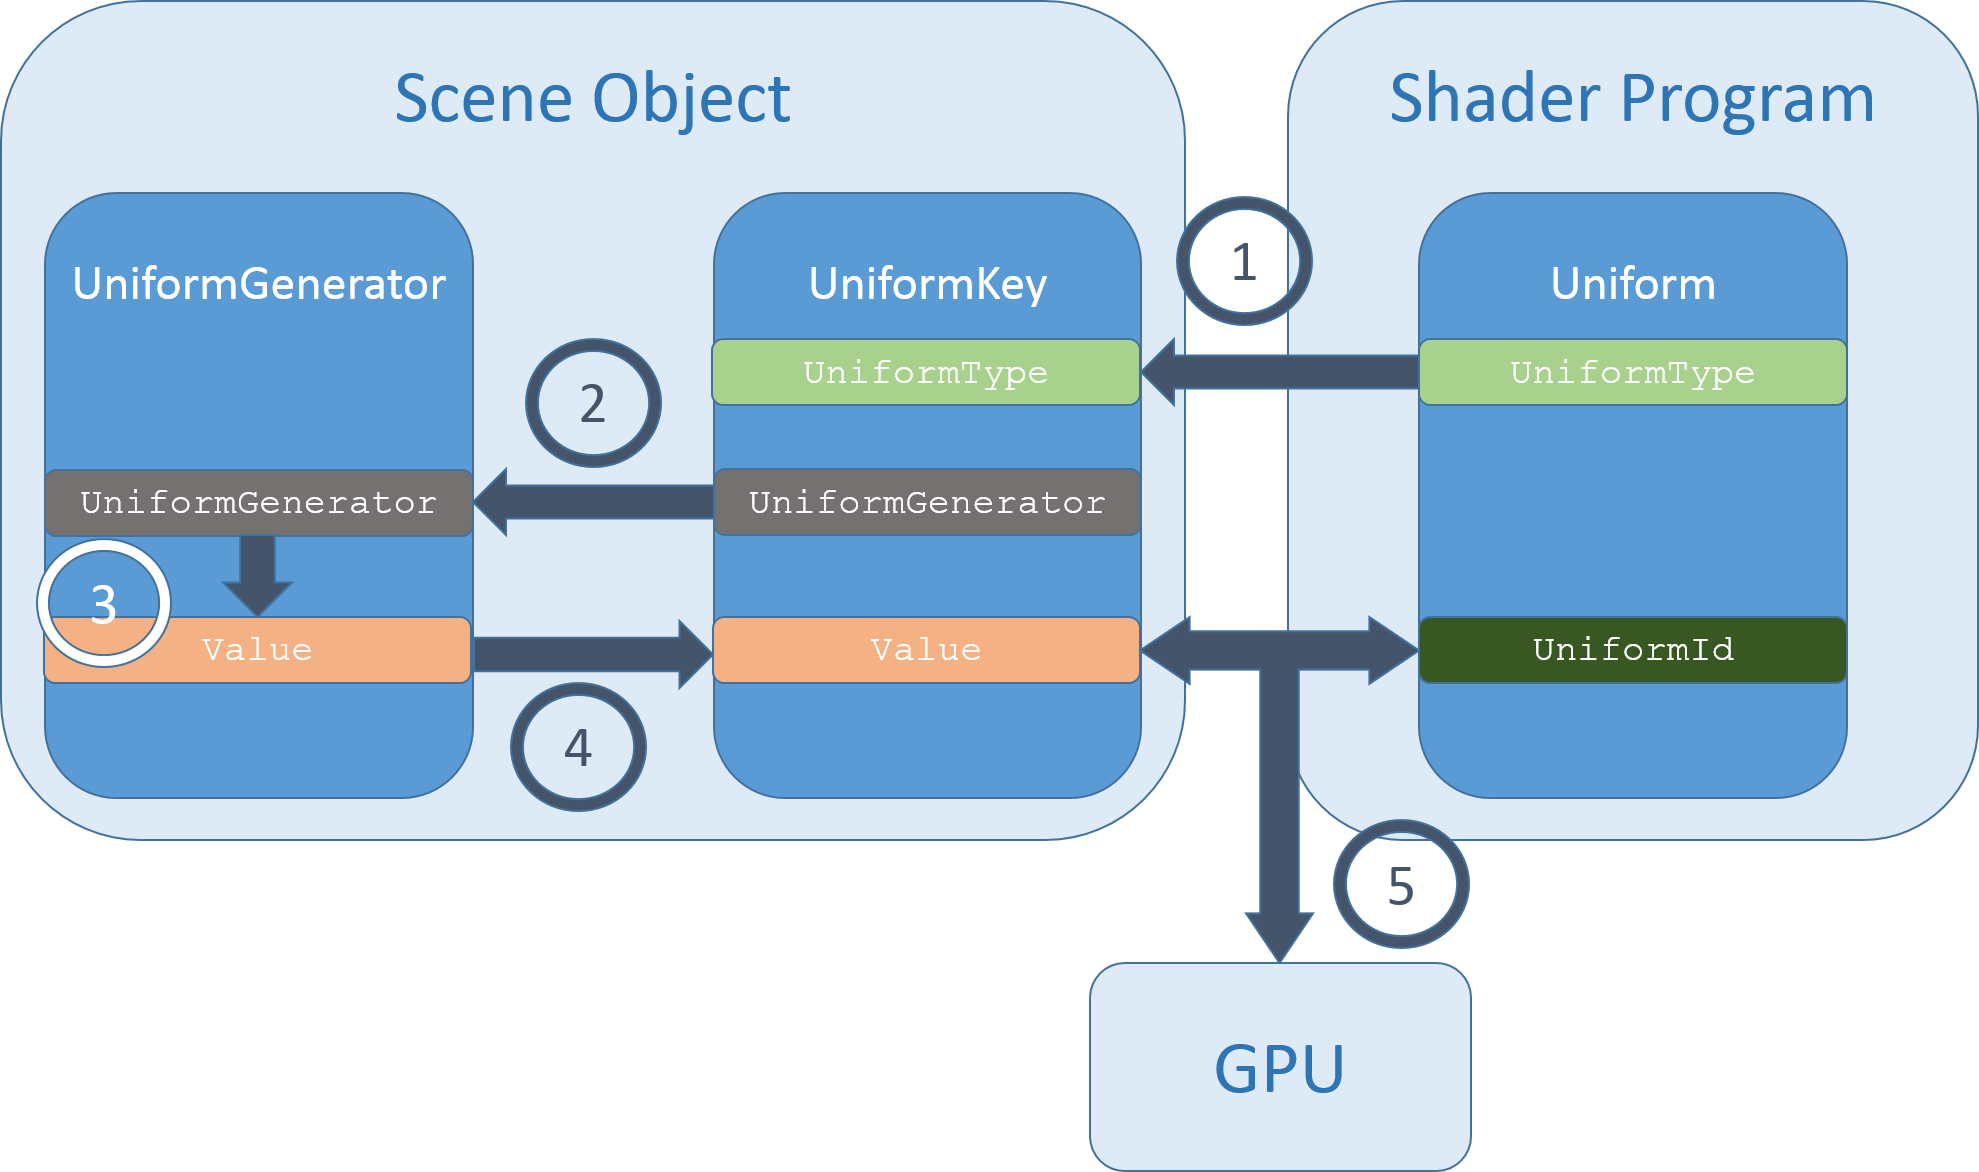
\includegraphics[scale=0.4]{uniformsgeneratorsandkeys.png}
\end{center}
\caption[Funcionamiento de UniformKeys y UniformsGenerators]{Funcionamiento de UniformKeys y UniformsGeneratos.\\
1. Búsqueda del objeto con el UniformType capaz de generar el Uniform dado.\\
2. Búsqueda dentro del objeto del UniformGenerator asociado al UniformKey.\\
3. Generación del valor del Uniform.\\
4. Almacenamiento del valor dentro del UniformKey.\\
5. Envío a la GPU el valor del Uniform generado.}
\label{fig:unifkeysandgen}
\end{figure}

De estos elementos, tanto Uniforms como UniformKeys son proporcionados por el fichero MRR como una parte más de un objeto, sin embargo, los UniformGenerators, son proporcionados vía código. Algunos de estos UniformGenerators, o al menos, los más usuales son provistos por el propio motor, sin embargo, la API ofrece la posibilidad de que el usuario pueda crear un nuevo UniformGenerator así como modificar el comportamiento de alguno ya existente tal y como se explica en.\\

Por último mencionar que los UniformGenerators pueden llegar a presentar un grave problema si no se controla. En el caso de que por ejemplo se necesitase calcular una cierta multiplicación de dos matrices $A$ y $B$ y que tanto $A$ como $B$ deben generarse también en un UniformGenerator. Ante esta situación podría pasar que $AB$ fuese calculada antes de generar las matrices $A$ y $B$ para ese frame. Es por eso que se hace necesario añadir ciertas restricciones a los UniformGenerators, estos son los denominados niveles.\\
El nivel del UniformGenerator indica el orden en el que este debe ser calculado y va desde 0 en adelante.\\
En el ejemplo anterior $A$ y $B$ podrían tener niveles 0 ambas mientras que $AB$ podría estar en el nivel 1, de esta forma se asegura que tanto $A$ como $B$ son generadas previamente a $AB$\\

\subsection{La Necesidad del Rendering Context}
El \textbf{Rendering Context} es el elemento encargado organizar y optimizar los datos utilizados al dibujar la escena.\\

Una de sus principales funcionalidades es la de controlar la lista de UniformKeys requeridos por cada objeto a la hora del renderizado.

Además también posee un papel vital de cara al rendimiento, pues es el encargado de minimizar los cambios de estados de la GPU. Esto se consigue por una parte realizando una ordenación previa de los objetos de la escena gracias al objeto denominado Rendering Sorter, que es capaz de minimizar el coste de los cambios de estados a realizar durante la generación de un frame, y por otra parte, controlando qué elementos se encuentran presentes en la GPU, tarea desempeñada por el Rendering Context.\\

Por ejemplo, se ordenan todos los modelos que posean la misma textura, esta se envía una única vez a la GPU y es usada por todos estos modelos de, de esa forma se minimizará el número de cambio de texturas.\\

\begin{figure}[h!]
\begin{center}
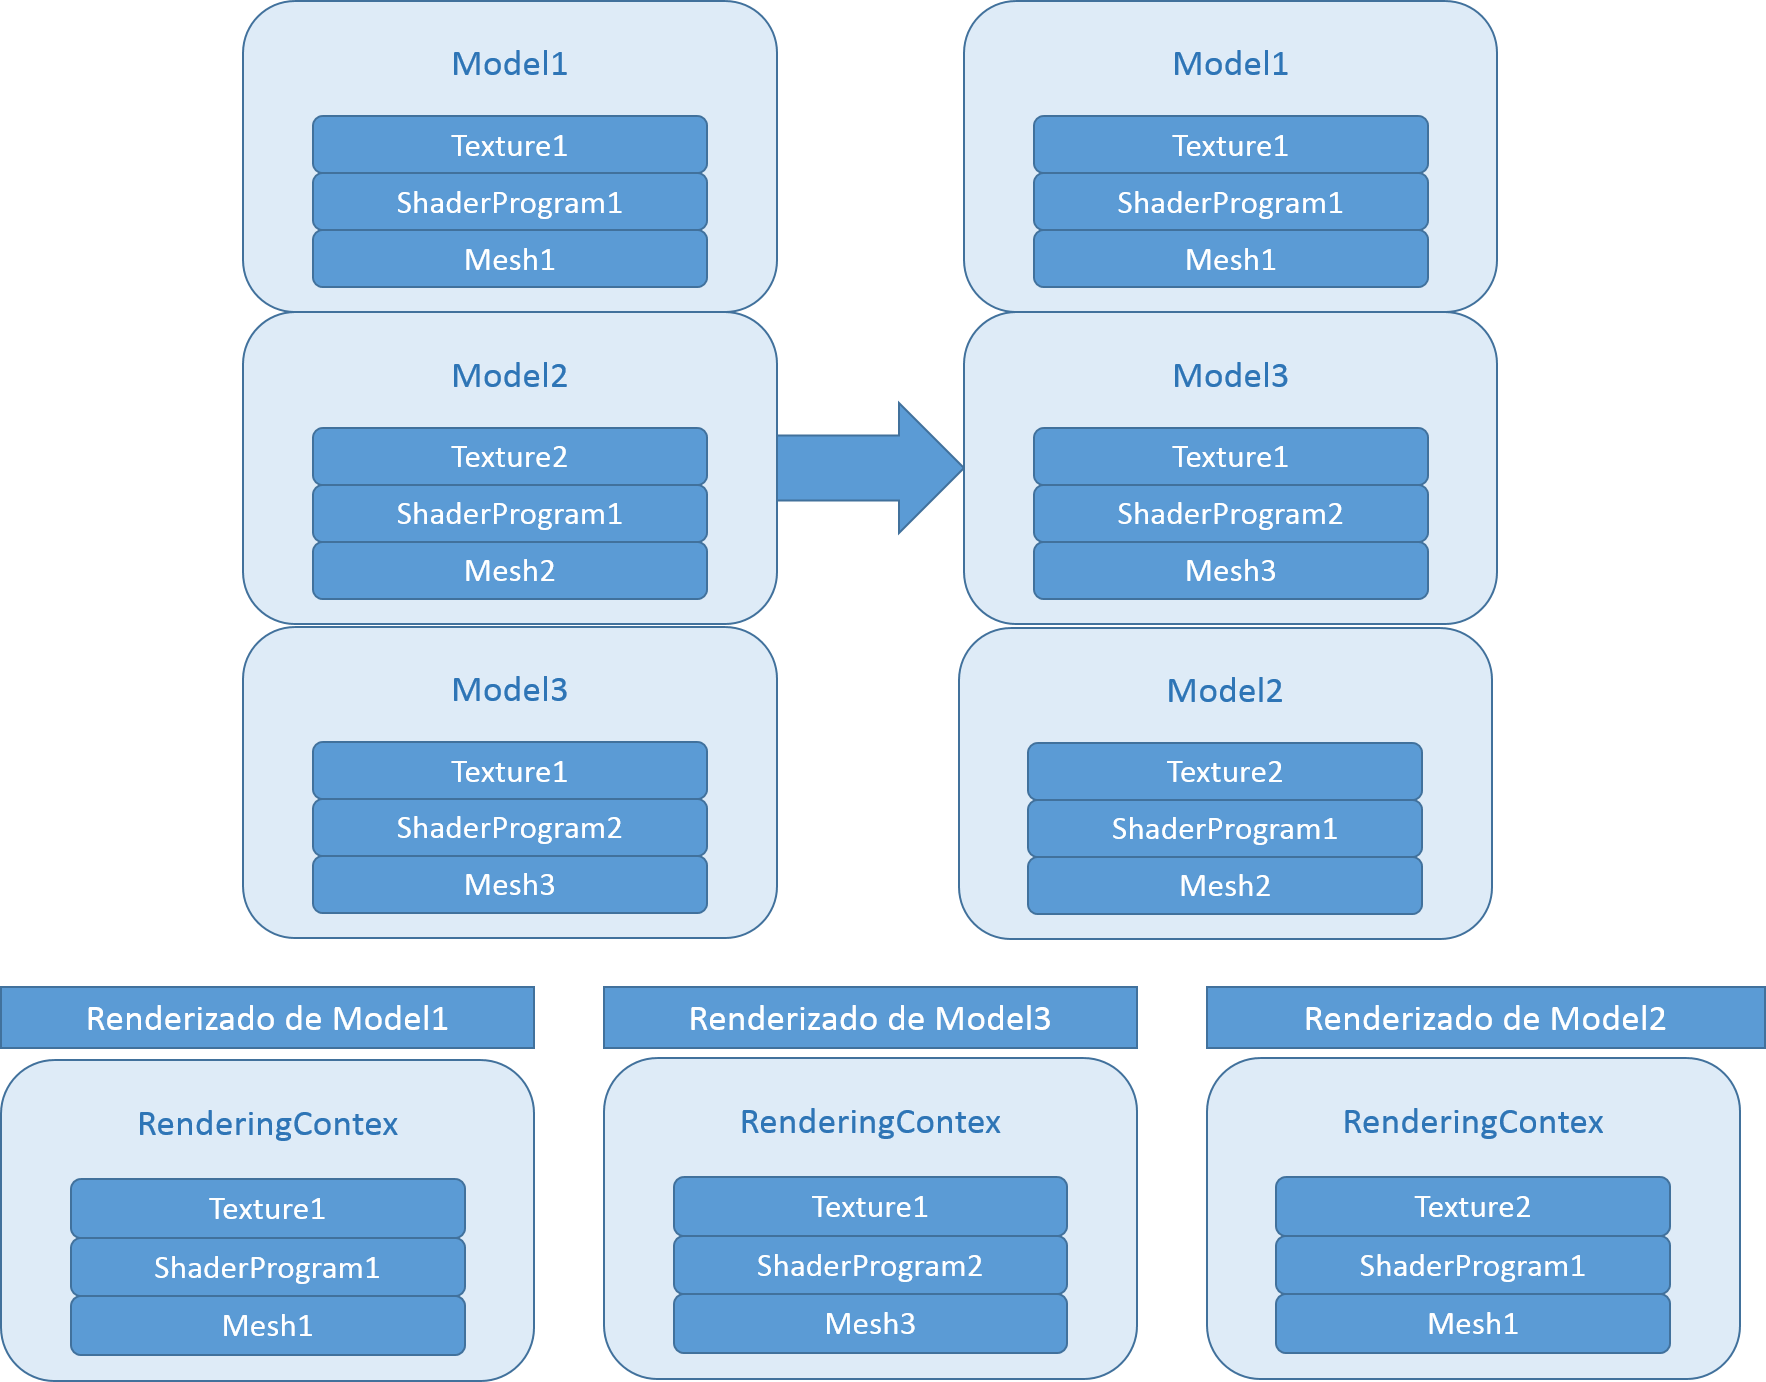
\includegraphics[scale=0.4]{renderingcontext.png}
\end{center}
\caption[Ejemplo del funcionamiento del Rendering Context]{Ejemplo del funcionamiento del Rendering Context}
\label{fig:renderingcontext}
\end{figure}

Un ejemplo del funcionamiento del Rendering Context en conjunto con el Rendering Sorter puede verse en la figura \ref{fig:renderingcontext}.\\
De proceder a renderizar los objetos en el orden predeterminado: Model1, Model2 y Model3 hay que notar que se establece en primer lugar Texture1, luego Texture2 y por último Texture1 de nuevo. Como se ha dicho, cambios de una textura a otra resultan operaciones costosas, así que se reorganizan los objetos de forma que al renderizar en el orden Model1, Model3 y Model2 únicamente se produce un cambio de estado en la textura en lugar de dos.

\subsection{Eventos}
Los eventos dentro de \robotto son implementados en dos partes, en primer lugar el dispositivo registra un evento procedente del exterior como podría ser que el usuario tocase la pantalla, o incluso este evento puede proceder del propio \robotto, como podría ser el evento \textit{Tick} que indica que se produce una llamada para generar un frame.\\

Una vez estos eventos se detectan se les asigna un identificador único y además almacenan los datos recibidos en el evento.\\

Ahora bien, los eventos no se ejecutarán de forma sincronizada con \robotto, es necesario buscar algún mecanismo de sincronización entre la ejecución de la aplicación que produce los eventos, y la ejecución de la renderización. Para ello lo que se ha decidido hacer es compartir una cola de eventos entre distintos hilos de ejecución, de esa forma cuando un evento es recibido este se envía a la cola compartida, y cuando se ejecute la renderización se procederá a procesar los elementos 
en orden de llegada.\\

Finalmente, y cuando sean procesados uno a uno los eventos la información almacenada en ellos será delegada a los distintos eventos que sean responsables del tratamientos de estos.\\

\subsection{Algoritmo de Renderizado}
Ahora que se han tratado todos los conceptos fundamentales que definen el funcionamiento del motor se puede establecer el comportamiento del ciclo del renderizado desde su inicialización hasta la generación de la imagen final.\\

En primer lugar se presenta el esquema de inicialización de los elementos gráficos.\\
Como se puede apreciar en primer lugar se inicializan todos los objetos uno a uno, se hacen llamadas a la GPU como podrían ser compilaciones de Shader Programs o configuración de texturas,
tras ello se acude al RenderingSorter, encargado de ordenar los objetos de la escena en función del coste de los cambios de estado en la GPU.\\
Finalmente se realizan las inicializaciones que requieran conocer el tamaño de la ventana 

\begin{figure}[h!]
\begin{center}
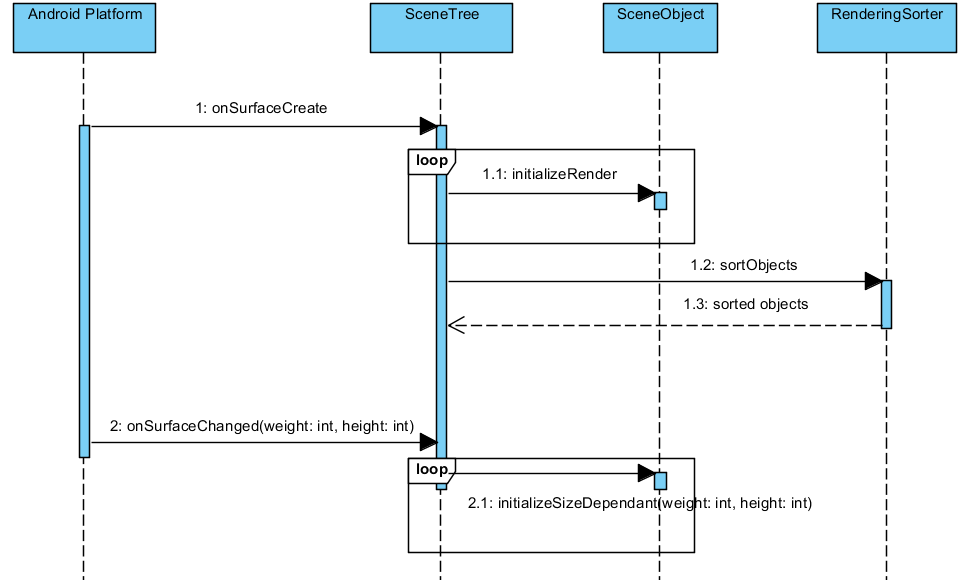
\includegraphics[scale=0.6]{initrender.png}
\end{center}
\caption[Inicialización de Recursos para el Renderizado]{Inicialización de Recursos para el Renderizado}
\label{fig:initrender}
\end{figure}

En el caso del renderizado de un frame lo primero que se realiza es actualizar el objeto según los eventos recibidos.\\
Tras ello tomamos el primer modelo de la lista de modelos ordenados generados en la inicialización y cargamos en la lista de UniformKeys todos los UniformKeys de este modelo y del resto de objetos activos, a saber: la cámara actual, las luces y la escena.\\
Una vez todos los UniformKeys han sido ordenados por nivel de dependencias se generan los valores de estos en los UniformGenerators y se envían a la GPU.

\begin{figure}[h!]
\begin{center}
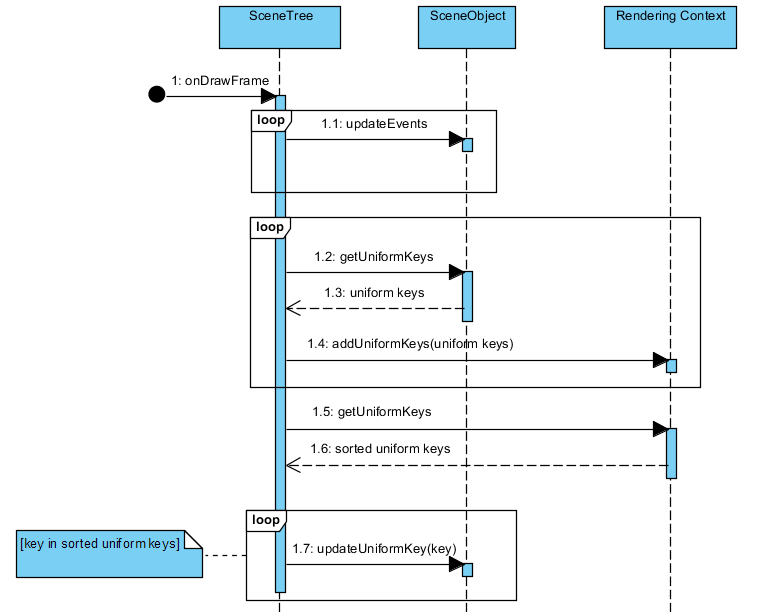
\includegraphics[scale=0.7]{renderrender.png}
\end{center}
\caption[Renderizado de un Frame]{Renderizado de un Frame}
\label{fig:renderrender}
\end{figure}




%-----------------------------------
%	SECTION 2
%-----------------------------------
\section{Arquitectura de \robotto}

\subsection{Interfaz de Uso}

\begin{figure}[h!]
\begin{center}
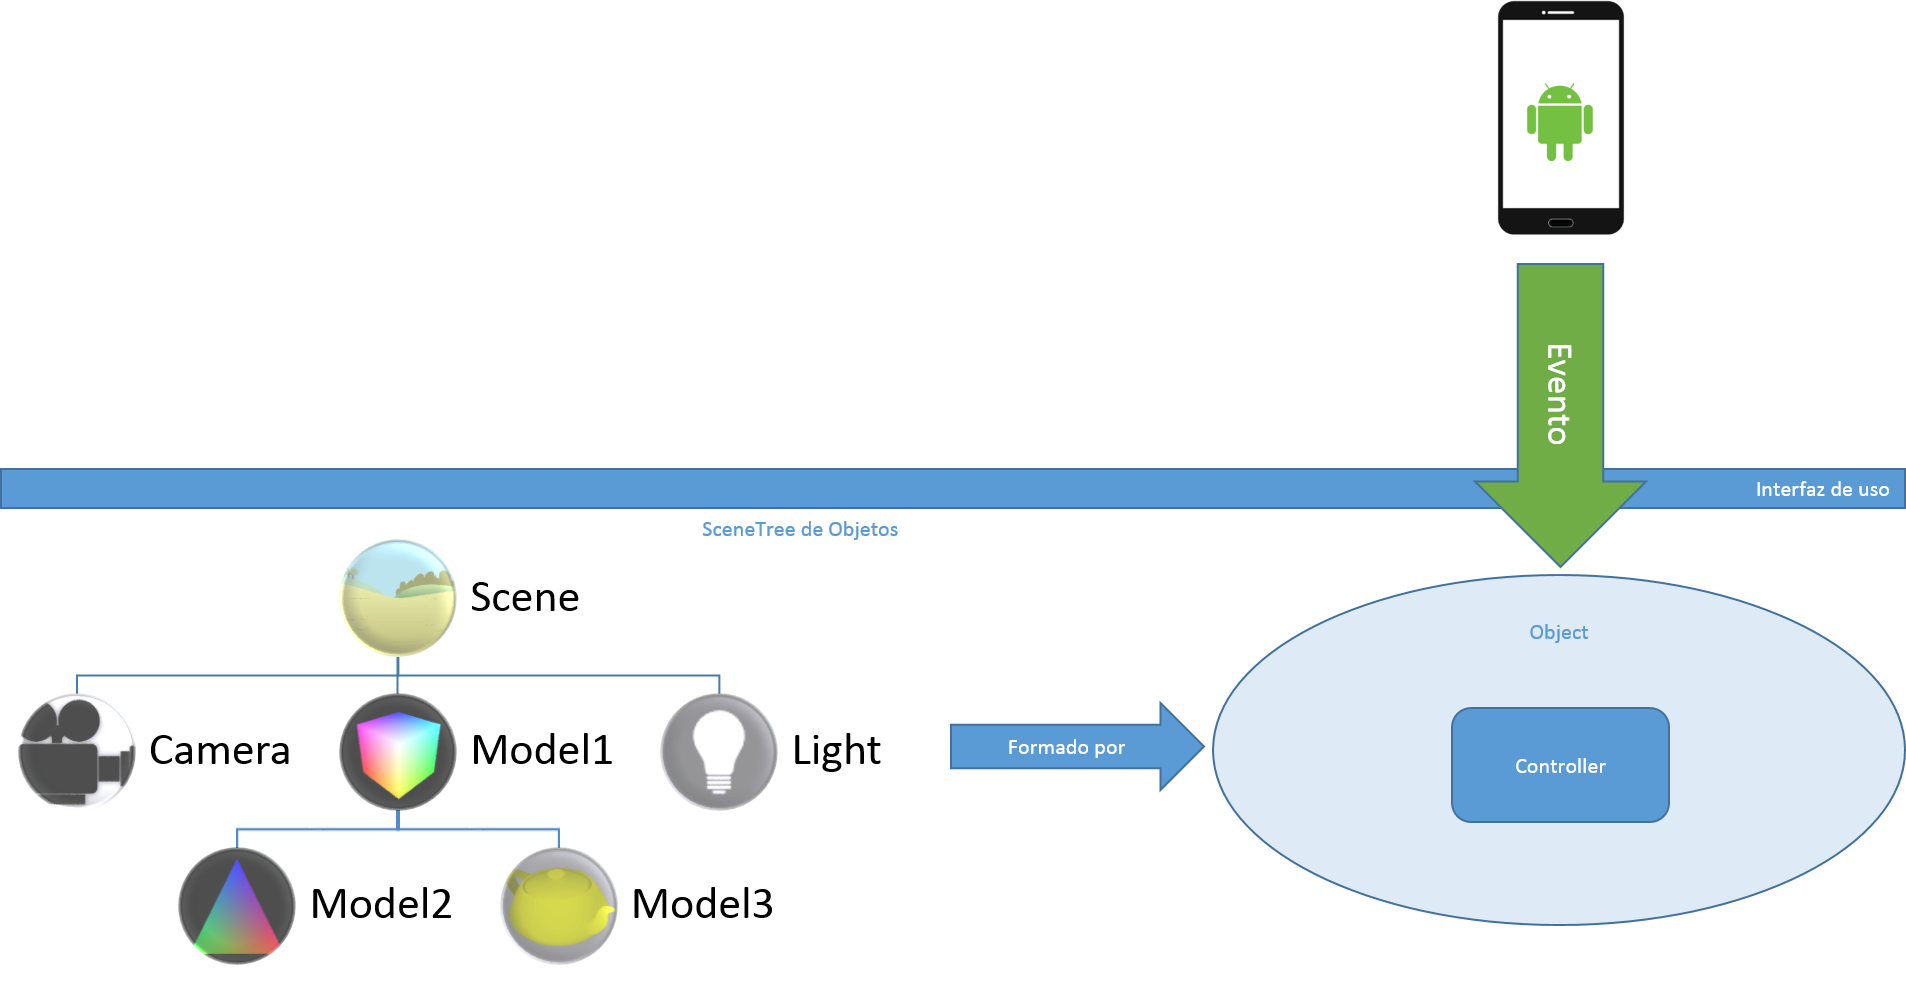
\includegraphics[scale=0.4]{interfaznucleo.png}
\end{center}
\caption[Interfaz del núcleo]{Interfaz del núcleo}
\label{fig:interfaznucleo}
\end{figure}

La interfaz de uso está compuesta por los elementos pensados para ser usados por los usuarios de \robotto.\\
Dichos elementos proveen al usuario de acciones comunes al tratar con objetos en una escena 3D como por ejemplo trasladar un objeto, rotarlo, ejecutar una animación,... U otras funcionalidades más generales como la búsqueda de objetos dentro de una escena, control de la jerarquía o de gestión de eventos.\\
Además, dichas herramientas son gestionadas de forma muy similar a como se gestiona el ciclo de vida de las aplicaciones Android comúnes, permitiendo mantener un paradigma similar al de la plataforma sobre la que se trabaja, intentando así que el usuario se sienta lo más cómodo posible a la hora de integrar \robotto en su aplicación.\\

\subsubsection{Integración en una Aplicación Android}

A la hora de integrar \robotto dentro de una aplicación Android \rorefrobottoengine\label{ro:robottoengine} es sin duda el primer objeto con el que se encuentra el usuario al usar \robotto. Es el encargado de la gestión del ciclo de vida de este, así como el encargado de gestionar los recursos usados y referencias a estos.\\
\begin{center}
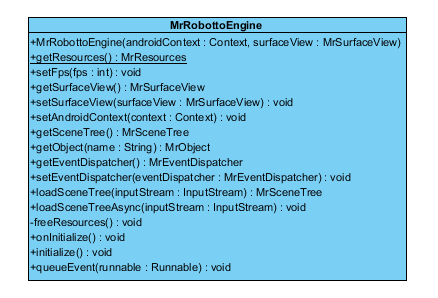
\includegraphics[scale=0.7]{mrrobottoengine.png}
\end{center}

Para inicializar una instancia de esta clase el usuario requerirá por una parte de un \textit{Context} de la plataforma Android, como podría ser una \textit{Activity} y por otra una referencia a una instancia de \rorefsurfaceview\label{ro:surfaceview}, esta clase hereda de la clase \textit{View} de la plataforma Android y será donde se mostrará el contenido.\\

Una vez se ha obtenido una referencia a un objeto de la clase \rorefrobottoengine el siguiente paso consiste en cargar una escena desde un \textit{stream} de datos. Este \textit{stream} de datos ha de contener datos en el formato MRR.\\
La carga de estos datos puede realizarse de dos formas distintas, de forma bloqueante o de forma no bloqueante, para ello se usarán los métodos \rorefm{MrRobottoEngine}{loadSceneTree-java.io.InputStream-}{loadSceneTree} y \rorefm{MrRobottoEngine}{loadSceneTreeAsync-java.io.InputStream-}{loadSceneTreeAsync} respectivamente.\\

Cuando la carga de datos haya finalizado se llamará automáticamente al método \rorefm{MrRobottoEngine}{onInitialize--}{onInitialize}, este método está pensado para ser sobrescrito en clases que hereden de \rorefrobottoengine ya que proporciona un entorno seguro para acceder a la escena, sus objetos y proporcionar código de iniciación.\\

\subsection{Objetos de la Escena}
Una vez hemos cargado la escena que usaremos nos interesa conocer los distintos objetos que pueden utilizarse.\\

\subsubsection{MrSceneTree}\label{susec:MrSceneTree}
El objeto \rorefscenetree es la interfaz que se le ofrece al usuario para acceder a la escena.\\
Este es el punto de entrada a la hora de acceder a cualquier objeto.


\subsubsection{MrObject}
\rorefobject\label{ro:object} es la clase base de toda nuestra jerarquía y la que contiene los métodos más genéricos para el control de un objeto de la escena.\\
\begin{figure}[h!]
\begin{center}
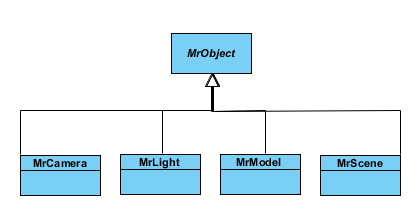
\includegraphics[scale=0.8]{robottohierarchy.png}
\end{center}
\caption[Jerarquía de MrObject]{Jerarquía de MrObject}
\label{fig:robottohierarchy}
\end{figure}
A pesar de ser una clase considerablemente importante de cara al uso, esta clase en realidad actúa como un envolvente de una clase de nivel inferior, \textit{MrObjectController}, de la que se hablará más adelante.\\

Las posibles acciones que se pueden realizar con una instancia de \rorefobject podrían dividirse en cuatro grupos según su funcionalidad.\\
Estas son o bien métodos genéricos, como podrían ser el constructor u obtener el tipo de objeto, métodos orientados a la gestión de eventos, como agregar o eliminar un evento a procesar, de jerarquía, como acceder a los hijos o al padre de un objeto, o de transformación, como puede ser rotar, escalar o trasladar el objeto.\\

\begin{figure}[h!]
\centering
\subfloat[Métodos Genéricos]{
  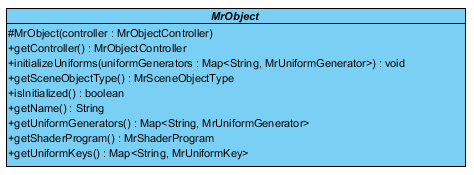
\includegraphics[scale=0.6]{objgeneric.png}
}
\subfloat[Métodos de Gestión de Eventos]{
  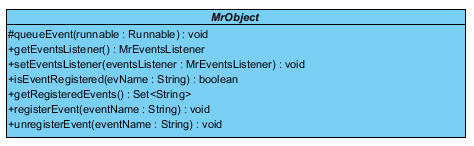
\includegraphics[scale=0.6]{objevents.png}
}
\hspace{0mm}
\subfloat[Métodos de Gestión de JerarQuía]{
  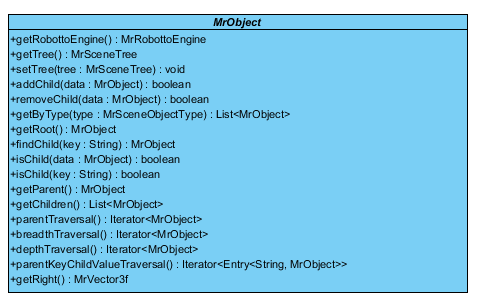
\includegraphics[scale=0.6]{objtree.png}
}
\subfloat[Métodos de Transformaciones Geométricas]{
  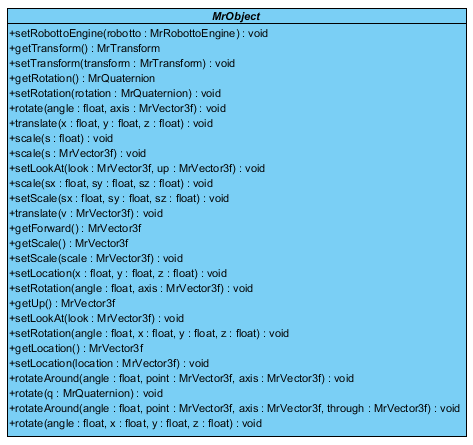
\includegraphics[scale=0.6]{objtransform.png}
}
\caption[Métodos de MrObject]{Métodos de MrObject agrupados por funcionalidad.}
\label{fig:metodosmrobject}
\end{figure}

El resto de tipos de objetos que pueden estar presentes en la escena, a saber: \rorefmodel, \rorefcamera, \roreflight y \rorefscene, comparten gran parte de la interfaz de \rorefobject, sin embargo, representan objetos de la escena los cuales tienen atributos únicos de su tipo.\\ 

\subsection{Eventos}

La gestión de los eventos a nivel interno se realiza en dos pasos.\\
El primero de ellos reside sobre la clase \rorefeventdispatcher pues es la encargada de recibir los eventos desde su fuente y tras ello enviarlo para su procesado dentro del bucle principal de renderización.\\
Dichos eventos deben establecer un identificador único para distinguir el tipo de evento enviado.\\
Además, a veces resulta necesario el envío de datos captados del evento se ha diseñado un elemento denominado \rorefbundle, en este elemento un usuario que reimplementase el comportamiento del \rorefeventdispatcher asociado al motor en ese momento debería hacer uso de esta herramienta para el envío de datos.\\

Una vez dichos datos llegan al hilo de ejecución del renderizado se procesan en orden de llegada para ser procesados dentro de los llamados \rorefeventlistener, estos elementos están asociados a cada uno de los objetos de la escena.\\
Ahora bien, no todos los objetos procesan todos los eventos recibidos, los \rorefeventlistener registran una serie de eventos a procesar, de esa forma, si un \rorefeventlistener tiene registrado el identificador de un cierto evento significa que será procesado por él, e ignorándolo en caso de que no esté registrado. En caso de que se procese el evento, el EventListener recibe como argumento la referencia al \rorefbundle asociado al evento recibido.

\subsection{Estructura de los Objetos}
Como se ha comentado ya durante este documento, la clase \rorefobject y todas sus subclases, son interfaces de una estructura subyacente encargada de administrar los objetos de la escena, tanto desde la gestión de eventos, pasando por el renderizado, como la gestión de los datos del objeto de la escena.\\
Dicha estructura podría verse compuesta por tres partes diferenciadas.

\begin{figure}[h!]
\begin{center}
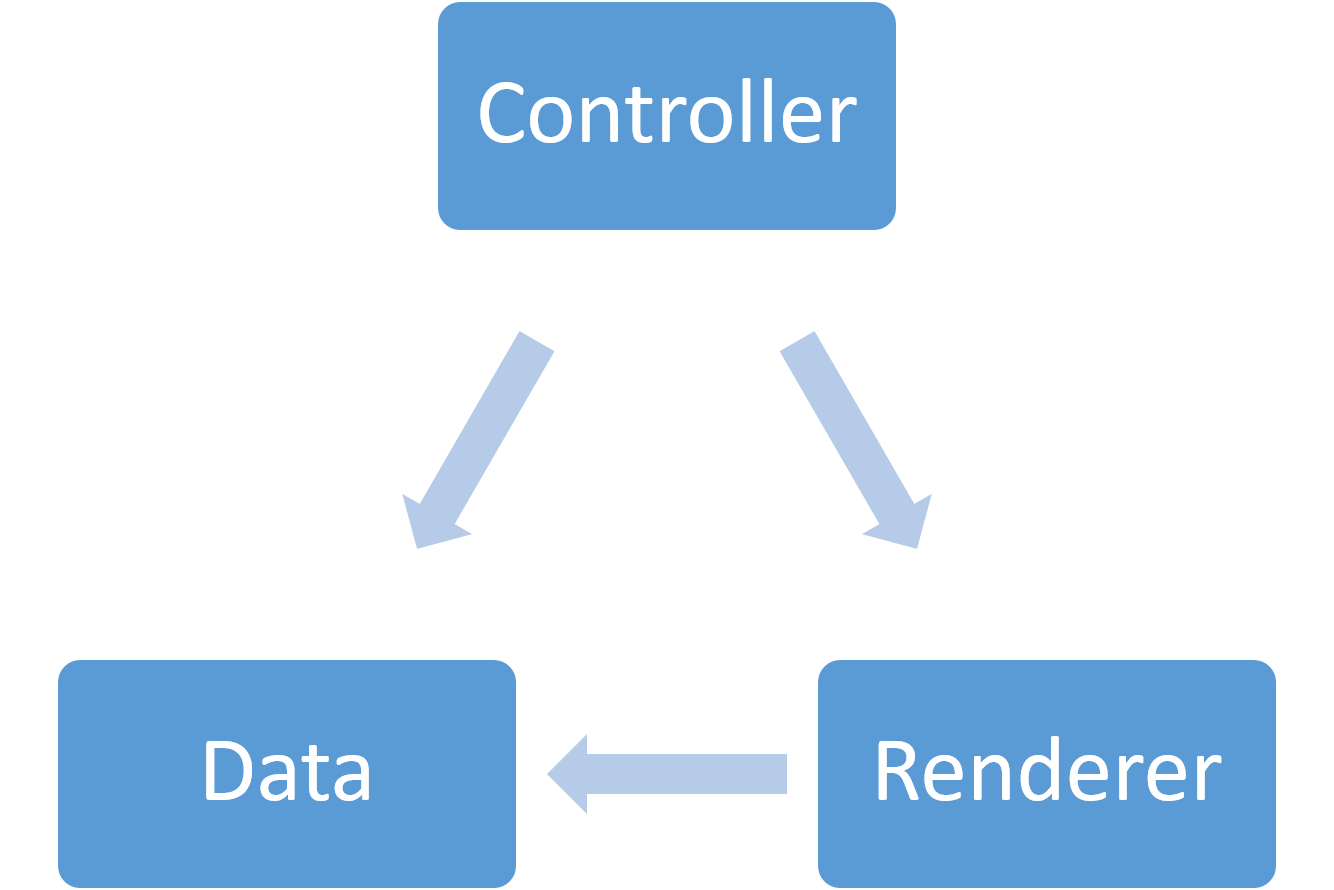
\includegraphics[scale=0.5]{mdr.png}
\end{center}
\caption[Estructura interna de los objetos]{Estructura interna de los objetos.}
\label{fig:mdr}
\end{figure}

Tal y como se puede apreciar en la figura \ref{fig:mdr} la estructura emula al patrón modelo-vista-controlador(MVC), y eso es precisamente lo que se buscaba, tres partes diferenciadas y cada una con unas responsabilidades definidas.

\subsubsection{Contenedores de Datos}
Los contenedores de datos serían la parte del modelo dentro del patrón MVC, su funcionalidad está restringida a almacenar datos necesarios del objeto que serán requeridos o bien por el controlador o bien por la parte del renderizador.\\
En los contenedores de datos también son almacenados tanto los UniformKeys de los objetos como los UniformGenerators que posean, y aunque su uso se realice mediante el controlador, este actúa como una interfaz.\\
Todos los elementos contenedores de datos requieren que se herede de la clase \rorefobjectdata\\
Todos los contenedores de datos se encuentran dentro del paquete \roref{engine/core/data/package-summary}{mr.robotto.engine.core.data}
\subsubsection{Renderizadores}
Los renderizadores hacen la función de la vista dentro del patrón MVC. Se encargan de tomar datos desde el modelo y presentarla como se requiera.\\
Los renderizadores están pensados para que todas las llamadas a OpenGL sean ejecutadas desde aquí, de esta forma todas las llamadas a la API se encontrarán concentradas en unas clases determinadas, lo cuál resulta muy beneficioso en cuanto a mantenibilidad de código se refiere.\\
Todos los objetos que se encarguen del renderizado deben implementar una cierta interfaz denominada \rorefobjectrender en la cuál es necesario implementar los siguientes métodos

\begin{itemize}
\item \texttt{void initializeRender(MrRenderingContext context, MrObjectData link)}\\
En este método al renderer se le asignan el rendering context sobre el cuál trabajará y además el objeto al que estará asociado.\\ 
Además en este método se inicia el objeto desde el punto de vista gráfico, es decir, se realizan tareas tales como configurar texturas, compilar Shader Programs y similares.
\item \texttt{void initializeSizeDependant(int w, int h)}\\
En este método se inician los recursos que dependan del tamaño de la ventana usada en ese momento.
\item \texttt{boolean isInitialized()}\\
Simplemente comprueba si el renderizador ha sido iniciado
\item \texttt{void render()}\\
Este método es el encargado de pasar datos a la tarjeta gráfica en cada frame.
\end{itemize}
Todos los renderizadores de objetos se encuentran dentro del paquete \roref{engine/core/render/package-summary}{mr.robotto.engine.core.render}
\subsubsection{Controladores}\label{rref:controlador}
La figura del controlador es la encargada de coordinar y dar sentido a todos los elementos que, en conjunto, conformen un objeto de la escena. 

\begin{figure}[h!]
\begin{center}
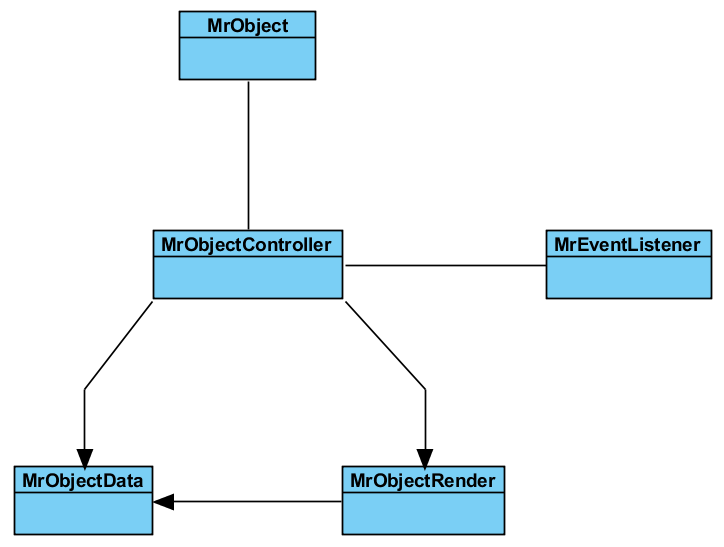
\includegraphics[scale=0.5]{controlleresquema.png}
\end{center}
\caption[Elementos destacables de MrObjectController]{Elementos destacables de MrObjectController}
\label{fig:controlleresquema}
\end{figure}

Como se puede apreciar en el esquema se comunican tanto con la capa de datos como la del renderizado, además proporciona un contexto válido a los \rorefobject y a los \rorefeventlistener.\\

Todos los controladores deben heredar de la clase \rorefobjectcontroller y se encuentran dentro del paquete \roref{engine/code/controller/package-summary}{mr.robotto.engine.core.controller}\\

\subsection{Componentes}
Los componentes son elementos especiales dentro de \robotto encargados de almacenar datos y comunicarse con la GPU.\\
Aunque los componentes puedan resultar similares en funcionalidad a los objetos de la escena la diferencia radica en que los componentes tienen un uso casi exclusivo a nivel interno del motor.\\
Los componentes además disfrutan de una estructura interna que sigue el patrón MVC, aunque en su caso, y por motivos de simplificación, la capa de datos y renderizado se han implementado como clases internas y siendo el controlador una interfaz a estas dos.\\

Así pues, la finalidad de estos elementos es la de conformar los atributos de la capa de datos de los objetos de la escena y simplificar el código del renderizado.\\

Todos los componentes deben heredar desde la clase base que se ha definido para este fin: \rorefcomponent

\subsection{MrModelController y sus Componentes}
Por su relevancia e interés se ha decidido hacer una mención especial a los modelos, que como componentes visibles que son, poseen una cierta relevancia que debe ser tratada en detalle.

\subsubsection{Mallas 3D}
Las mallas 3D, o como se han denominado en \robotto, \rorefmesh, son componententes pertenecientes a los modelos.\\
Son los encargados de enviar los datos relativos a los vértices a la GPU.\\
Para representar una malla harán falta dos elementos fundamentales:

\begin{itemize}
\item Los Vertex Buffer Objects (VBO), que son listas de datos numéricos encargados de almacenar la información de cada uno de los vértices, como las coordenadas donde se encuentra, las normales, el índice del material que usan,...
\item Los Index Buffer Objects (IBO), que son listas de índices que indican el orden en el que los vértices deben ser leídos.
\end{itemize}

Estos buffers en la implementación son los denominados \rorefbuffer.

Ahora bien, los VBOs representan los datos de una forma no estructurada y se requiere poder diferenciar los distintos datos contenidos en ellos, con este fin existen los \rorefbufferkey.\\
Los \rorefbufferkey son los encargados de determinar en qué índice del VBO empieza y acaba un dato específico de un vértice.\\
Dentro de sus atributos importantes están:
\begin{itemize}
\item \texttt{Pointer}: Índice del buffer de la primera aparición de un cierto dato.
\item \texttt{Size}: Tamaño del dato
\item \texttt{Stride}: Número de elementos el inicio de un cierto tipo de dato y su siguiente aparición.
\end{itemize}

Por ejemplo:\\
\begin{figure}[h!]
\begin{center}
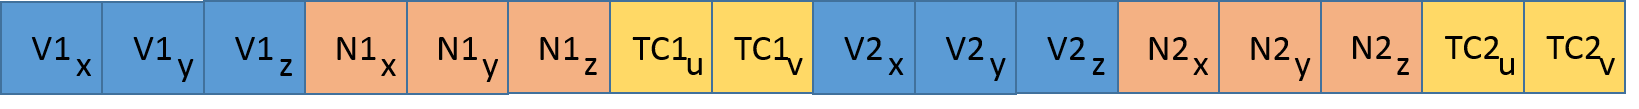
\includegraphics[scale=0.5]{interleaved2.png}
\end{center}
\caption[Estructura de un VBO]{Estructura de un VBO.\\ V representa las coordenadas del vértice, N su normal y TC sus coordenadas de textura}
\label{interleaved2}
\end{figure}

En la figura \ref{interleaved2} se aprecian tres tipos de datos almacenados en el buffer, luego sus valores de \texttt{Pointer}, \texttt{Size} y \texttt{Stride} son:
\begin{itemize}
\item Para las coordenadas:\\
Su \texttt{Pointer} es 0 ya que en el 0 tenemos su primera aparición, su \texttt{Size} es de 3, mientras que el \texttt{Stride} es de 8 ya que hasta la octava posición no vuelve a haber un bloque de coordenadas

\item Para las normales:\\
Su \texttt{Pointer} es 3, su \texttt{Size} es de 3, y su \texttt{Stride} es de 8.

\item Para las texturas:\\
Su \texttt{Pointer} es 6, su \texttt{Size} es de 2, y su \texttt{Stride} es de 8.
\end{itemize}

Así pues, gracias a estos dos objetos, \rorefbuffer y \rorefbufferkey, una malla tridimensional es capaz de enviar la información necesaria a los vértices a la GPU

\subsubsection{Materiales}
Los materiales son los elementos encargados de discernir como afecta la luz a la superficie de la malla. Y se encuentran definidos por la clase \rorefmaterial.\\

Cuando una luz actúa sobre una malla con un cierto material se usan los distintos atributos del material para determinar como este reaccionará ante la luz ambiental, difusa y especular. Por defecto en \robotto la reflexión de la luz se hace mediante \textit{Blinn-Phong} sin embargo el código fuente de los shaders puede modificarse y conseguir así otro tipo de reflexión como toon-shading por ejemplo.
 

\subsubsection{Texturas}
Las texturas son un componente opcional de los modelos y se encuentran altamente relacionadas con los materiales pues definen el aspecto de las mallas al ser renderizadas.\\
Las imágenes utilizadas como texturas proceden del fichero MRR y se almacenan en memoria. Una vez la textura asociada a una imagen es inicializada, y con ello, almacenada en memoria nativa, la imagen es liberada de los recursos del sistema.\\
Además, y ya que se trabaja sobre sistemas con pocos recursos, se recomienda que dichas imágenes sean siempre dentro de lo posible cuadradas, con lado de medida una potencia de dos y lo más pequeñas posibles. Las medidas usuales y recomendadas son de $256\times 256$ o $512\times 512$.\\

Las texturas vienen definidas dentro de la clase \roreftexture

\subsubsection{Animación}
La animación dentro de \robotto es la generada a partir de un esqueleto que afecte a la malla 3D.\\
Para conseguir esta funcionalidad se requieren múltiples elementos:\\

Por una parte hace falta un esqueleto, que consiste en un conjunto de huesos estructurados de forma jerárquica y donde cada uno actuará sobre un conjunto de vértices de la malla. Además el esqueleto es capaz de controlar las distintas animaciones que tiene asociadas, siendo capaz de proporcionar la localización y rotación de cada hueso a cada frame.\\
El esqueleto viene definido dentro de la clase \rorefskeleton y como ya se ha dicho se encuentra compuesto por huesos definidos en la clase \rorefbone.\\

Ahora bien, tal y como se ha comentado el esqueleto es capaz de controlar animaciones, pero para generar estas es necesario el uso de otras clases adicionales, estas son:

\begin{itemize}
\item Los \rorefframe almacenan los frames de la animación. Cada uno tiene una lista de huesos asociados y es la clase encargada de interpolar los keyframes importados de la animación al motor. 
\item La \rorefkeyframelist es la encargada de almacenar los keyframes importados de la animación. Y va generando los frames a medida que se solicitan. Si el keyframe existe porque ha sido exportado se da este, en otro caso, se interpola a partir del keyframe previo a él y el siguiente.
\item \rorefskeletalaction refleja una animación producida desde un esqueleto. Almacena la lista de keyframes y es la clase que se encuentra por debajo  
\end{itemize}

\subsubsection{Shader Program}
Unos de los componentes más importantes dentro de los modelos son los Shader Programs, pues son los encargados de mantener el código que se usará en la GPU a la hora de renderizar.

Se encuentra formada por tres elementos fundamentales:
\begin{itemize}
\item Attributes: Son la entrada de datos por cada vértice del Shader Program, en ellos se encuentran los datos enviados desde una malla 3D, y en el caso de los modelos, los Attributes se corresponden biyectivamente con los \rorefbufferkey de la malla del modelo.\\
Están representados por la clase \rorefattribute.
\item Uniforms: Los Uniforms son elementos que permanecen constantes para los conjuntos de vértices enviados en bloque a la CPU.\\
Almacenan un \texttt{UniformType} que es la constante que permite identificar de forma única al uniform dentro del shader.\\
Están definidos dentro de la clase \rorefuniform.
\item Shaders: Los Shaders por último son la clase que almacena el código que se ejecutará en la GPU. Los dos tipos posibles de Shaders implementados dentro de \robotto son los Vertex Shaders, encargados del procesado por vértice de una malla y los Fragment Shaders, encargados del procesado por pixel de la imagen generada.
\end{itemize}


\subsection{Paquete de Herramientas}
Entre las utilidades más relevantes para el funcionamiento de \robotto cabe destacar el papel de los cargadores de datos, encargados de transformar los ficheros \textit{".mrr"} a la estructura interna del motor, así como las distintas clases encargadas de representar estructuras de datos específicamente implementadas para acomodar los datos usados.

\subsubsection{Cargadores de Datos}
La carga de datos se podría distinguir en tres partes.\\
En primer lugar y como punto de entrada la carga del MRR file del que se encarga la clase \rorefmrrloader que se encarga de separar la sección JSON de la sección de las texturas.\\
Una vez separadas los bitmaps procedentes de las texturas se almacenan dentro de una instancia de la clase \rorefresources, que se trata de una clase auxiliar usada durante la carga de datos a modo de almacenamiento de recursos temporales o compartidos.\\
Por otra parte, durante el procesamiento de la sección JSON se pasa la información a la clase \rorefrobottojsonloader, en ella el trabajo se irá delegando de forma continua en clases especializadas, esto quiere decir que habrá un cargador de datos por cada sección de datos relevante, por ejemplo, podremos encontrar cargadores para los modelos, las luces o las cámaras ya que requieren un tratamiento distinto y generan un resultado distinto. Es por eso que todas estas clases en las que se delegan extienden la clase genérica \rorefjsonbaseloader, que proporciona una interfaz unificada y directa para la obtención de los datos. 

\subsection{Paquete de Estructuras de Datos}
Para la implementación de partes esenciales de la arquitectura, como por ejemplo, la construcción de la propia escena, se requerían de ciertas estructuras de datos específicas para la aplicación.\\
Este es el caso de \roreftreemap, clase encargada de presentar una estructura de árbol con un número variable de hijos por cada nodo y con capacidad de realizar búsquedas en el árbol de forma inmediata gracias a su diccionario interno.\\
Sobre esta clase están basados los árboles de la escena.\\

Ahora bien, como es necesario que estas clases posean una API sencilla de utilizar y a la vez una velocidad de acceso muy alta se ha desarrollado una herramienta auxiliar denominada \rorefmapfunction.\\
Esta sencilla clase permite realizar un mapeo directo entre los objetos contenidos en las estructuras y las llaves asociadas a ellos.\\
En el caso del Scene Tree este mapeo de datos es el que se origina de asignarle a cada objeto su nombre como llave.

\subsection{Paquete Matemático}
El paquete matemático de \robotto es posiblemente uno de los paquetes con más peso dentro de la aplicación. Es por ello que se ha invertido una gran cantidad de tiempo en su optimización y en que sea sencillo de usar.\\

La interfaz base para todos los objetos matemáticos dentro de \robotto es la denominada \roreflinearalgebra, su método más importante es posiblemente el método \texttt{float[] getValues} que es el encargado final de transmitir los datos almacenados en él hacia los Uniforms dentro de los Shader Programs.\\

Dependiendo de esta interfaz se encuentran clases usuales dentro de las aplicaciones 3D, a saber:

\begin{itemize}
\item Matrices 4x4: Encargadas de representar transformaciones lineales dentro del espacio tridimensional usando coordenadas homogéneas.\\
Las matrices 4x4 están representada por la clase \rorefmatrix
\item Cuaterniones: Orientados hacia las rotaciones\\
Los cuaterniones está representada por la clase \rorefquaternion dentro del motor.
\item Vectores de 3 y 4 componentes: Usados para representar puntos en el espacio, direcciones e incluso colores almacenados como RGB o RGBA.\\
Los vectores de 3 y 4 componentes vienen representados por las clases \rorefvectortresf y \rorefvectorcuatrof respectivamente.
\end{itemize}

Sobre estas clases fundamentales que son capaces de representar las transformaciones comunes del espacio tridimensional se fundamenta la clase \roreftransform, clase con un gran peso dentro de \robotto pues es la encargada de gestionar todas las transformaciones de un objeto de la escena.\\
Lleva a cabo transformaciones simples como rotar, trasladas o escalar, pero a su vez también se encarga de operaciones más complejas como la de rotar alrededor de un eje arbitrario y pasando por un cierto punto, rotar alrededor de un punto,...\\
Además otra de sus funciones es la de mantener un sistema de coordenadas locales del objeto, permitiendo tener una referencia de conceptos como qué es "ir hacia adelante o ir hacia arriba" para un objeto independientemente de las coordenadas del mundo.\\

Por otra parte, y como ya se ha mencionado, esta sección se encuentra altamente optimizada. Los métodos de operaciones matemáticas requieren de forma obligatoria que se les inyecte una instancia de la clase resultante, de esta forma se consigue delegar en un nivel superior la gestión de la memoria.\\
El por qué de esto se debe a que resulta altamente costoso el hecho de, por ejemplo, multiplicar dos matrices y tener que crear una nueva instancia cuando se devuelve el resultado, y más aún si consideramos que gran parte de esas operaciones se producen en cada frame.